% Codigo do grafico de trajetorias para o Experimento 2
\begin{figure}[H]
\centering
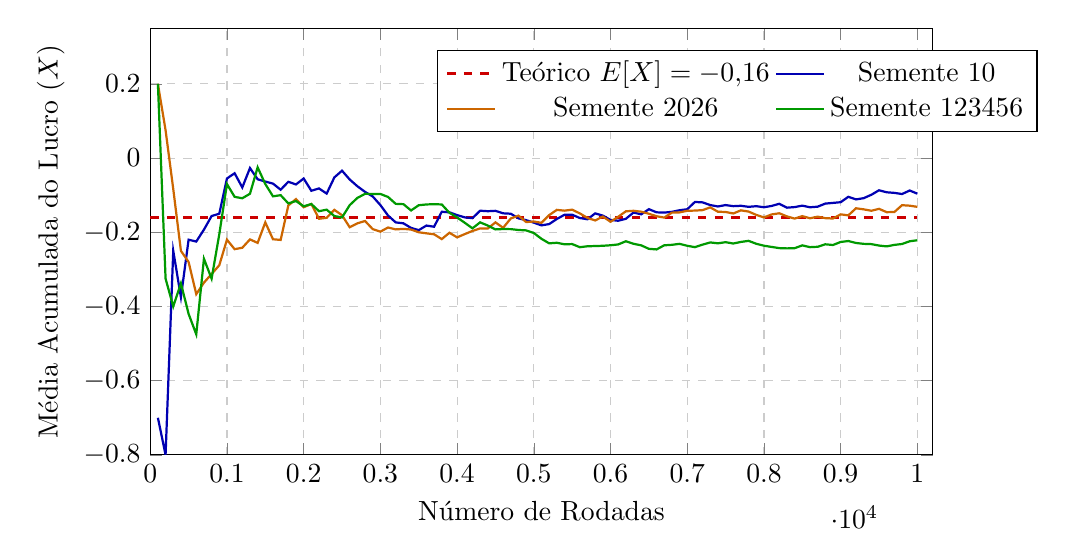
\begin{tikzpicture}
\begin{axis}[
    width=0.95\textwidth,
    height=7cm,
    xlabel={Número de Rodadas},
    ylabel={Média Acumulada do Lucro ($X$)},
    xmin=0, xmax=10200,
    ymin=-0.8, ymax=0.35,
    legend style={at={(0.75,0.95)}, anchor=north, legend columns=2},
    grid=major,
    major grid style={dashed, gray!40}
]

% Linha teorica de esperança E[X] = -0.16
\addplot[red!80!black, dashed, line width=1.3pt, domain=0:10000] {-0.16};
\addlegendentry{Teórico $\mathbb{E}[X] = -0{,}16$}

% Trajetoria Semente 10
\addplot[blue!70!black, thick] coordinates {
    (100, -0.7)
    (200, -0.8)
    (300, -0.25)
    (400, -0.375)
    (500, -0.22)
    (600, -0.225)
    (700, -0.1929)
    (800, -0.1562)
    (900, -0.15)
    (1000, -0.055)
    (1100, -0.0409)
    (1200, -0.0792)
    (1300, -0.0269)
    (1400, -0.0571)
    (1500, -0.0633)
    (1600, -0.0688)
    (1700, -0.0853)
    (1800, -0.0639)
    (1900, -0.0711)
    (2000, -0.055)
    (2100, -0.0881)
    (2200, -0.0818)
    (2300, -0.0957)
    (2400, -0.0521)
    (2500, -0.034)
    (2600, -0.0577)
    (2700, -0.0759)
    (2800, -0.0911)
    (2900, -0.1034)
    (3000, -0.1267)
    (3100, -0.1548)
    (3200, -0.1734)
    (3300, -0.1758)
    (3400, -0.1882)
    (3500, -0.1943)
    (3600, -0.1819)
    (3700, -0.1851)
    (3800, -0.1447)
    (3900, -0.1462)
    (4000, -0.1537)
    (4100, -0.1598)
    (4200, -0.1619)
    (4300, -0.1419)
    (4400, -0.1432)
    (4500, -0.1422)
    (4600, -0.1489)
    (4700, -0.15)
    (4800, -0.1625)
    (4900, -0.1673)
    (5000, -0.174)
    (5100, -0.1814)
    (5200, -0.1779)
    (5300, -0.1642)
    (5400, -0.1528)
    (5500, -0.1527)
    (5600, -0.1616)
    (5700, -0.1649)
    (5800, -0.1491)
    (5900, -0.1551)
    (6000, -0.1667)
    (6100, -0.1689)
    (6200, -0.1637)
    (6300, -0.1468)
    (6400, -0.1516)
    (6500, -0.1377)
    (6600, -0.1462)
    (6700, -0.147)
    (6800, -0.1449)
    (6900, -0.1406)
    (7000, -0.1379)
    (7100, -0.1183)
    (7200, -0.1194)
    (7300, -0.1267)
    (7400, -0.1304)
    (7500, -0.1267)
    (7600, -0.1296)
    (7700, -0.1286)
    (7800, -0.1314)
    (7900, -0.1297)
    (8000, -0.1325)
    (8100, -0.129)
    (8200, -0.1232)
    (8300, -0.1337)
    (8400, -0.1321)
    (8500, -0.1282)
    (8600, -0.1326)
    (8700, -0.131)
    (8800, -0.1227)
    (8900, -0.1208)
    (9000, -0.1189)
    (9100, -0.1044)
    (9200, -0.1114)
    (9300, -0.1081)
    (9400, -0.0989)
    (9500, -0.0868)
    (9600, -0.0922)
    (9700, -0.0938)
    (9800, -0.0969)
    (9900, -0.0874)
    (10000, -0.096)
};
\addlegendentry{Semente 10}

% Trajetoria Semente 2026
\addplot[orange!80!black, thick] coordinates {
    (100, 0.2)
    (200, 0.075)
    (300, -0.0833)
    (400, -0.25)
    (500, -0.28)
    (600, -0.3667)
    (700, -0.3357)
    (800, -0.3125)
    (900, -0.2889)
    (1000, -0.22)
    (1100, -0.2455)
    (1200, -0.2417)
    (1300, -0.2192)
    (1400, -0.2286)
    (1500, -0.1733)
    (1600, -0.2188)
    (1700, -0.2206)
    (1800, -0.1278)
    (1900, -0.1105)
    (2000, -0.1325)
    (2100, -0.1238)
    (2200, -0.1636)
    (2300, -0.1609)
    (2400, -0.1396)
    (2500, -0.154)
    (2600, -0.1865)
    (2700, -0.1759)
    (2800, -0.1696)
    (2900, -0.1914)
    (3000, -0.1983)
    (3100, -0.1871)
    (3200, -0.1922)
    (3300, -0.1909)
    (3400, -0.1926)
    (3500, -0.2)
    (3600, -0.2028)
    (3700, -0.2054)
    (3800, -0.2184)
    (3900, -0.2013)
    (4000, -0.2137)
    (4100, -0.2049)
    (4200, -0.1964)
    (4300, -0.1895)
    (4400, -0.1898)
    (4500, -0.1733)
    (4600, -0.188)
    (4700, -0.1628)
    (4800, -0.1552)
    (4900, -0.1724)
    (5000, -0.171)
    (5100, -0.1745)
    (5200, -0.1538)
    (5300, -0.1396)
    (5400, -0.1417)
    (5500, -0.1391)
    (5600, -0.1491)
    (5700, -0.1614)
    (5800, -0.1681)
    (5900, -0.1576)
    (6000, -0.1717)
    (6100, -0.1582)
    (6200, -0.1435)
    (6300, -0.1421)
    (6400, -0.1445)
    (6500, -0.15)
    (6600, -0.1568)
    (6700, -0.1604)
    (6800, -0.1471)
    (6900, -0.1464)
    (7000, -0.1421)
    (7100, -0.1415)
    (7200, -0.1403)
    (7300, -0.1329)
    (7400, -0.1446)
    (7500, -0.1453)
    (7600, -0.1493)
    (7700, -0.1409)
    (7800, -0.1442)
    (7900, -0.1532)
    (8000, -0.16)
    (8100, -0.1519)
    (8200, -0.1488)
    (8300, -0.1572)
    (8400, -0.1631)
    (8500, -0.1565)
    (8600, -0.1622)
    (8700, -0.158)
    (8800, -0.1619)
    (8900, -0.1629)
    (9000, -0.1517)
    (9100, -0.1544)
    (9200, -0.1353)
    (9300, -0.1382)
    (9400, -0.142)
    (9500, -0.1368)
    (9600, -0.1458)
    (9700, -0.1454)
    (9800, -0.127)
    (9900, -0.1283)
    (10000, -0.1315)
};
\addlegendentry{Semente 2026}

% Trajetoria Semente 123456
\addplot[green!60!black, thick] coordinates {
    (100, 0.2)
    (200, -0.325)
    (300, -0.4)
    (400, -0.3375)
    (500, -0.42)
    (600, -0.475)
    (700, -0.2714)
    (800, -0.325)
    (900, -0.2056)
    (1000, -0.07)
    (1100, -0.1045)
    (1200, -0.1083)
    (1300, -0.0962)
    (1400, -0.025)
    (1500, -0.07)
    (1600, -0.1031)
    (1700, -0.1)
    (1800, -0.1222)
    (1900, -0.1158)
    (2000, -0.13)
    (2100, -0.1238)
    (2200, -0.1432)
    (2300, -0.1391)
    (2400, -0.1562)
    (2500, -0.16)
    (2600, -0.1269)
    (2700, -0.1074)
    (2800, -0.0964)
    (2900, -0.0966)
    (3000, -0.0967)
    (3100, -0.1048)
    (3200, -0.1234)
    (3300, -0.1242)
    (3400, -0.1412)
    (3500, -0.1271)
    (3600, -0.125)
    (3700, -0.1243)
    (3800, -0.125)
    (3900, -0.1474)
    (4000, -0.16)
    (4100, -0.1744)
    (4200, -0.1893)
    (4300, -0.1733)
    (4400, -0.1818)
    (4500, -0.1922)
    (4600, -0.1913)
    (4700, -0.1915)
    (4800, -0.1938)
    (4900, -0.1949)
    (5000, -0.202)
    (5100, -0.2176)
    (5200, -0.2298)
    (5300, -0.2283)
    (5400, -0.2324)
    (5500, -0.2318)
    (5600, -0.2402)
    (5700, -0.2377)
    (5800, -0.2371)
    (5900, -0.2364)
    (6000, -0.235)
    (6100, -0.2328)
    (6200, -0.2242)
    (6300, -0.231)
    (6400, -0.2352)
    (6500, -0.2446)
    (6600, -0.2462)
    (6700, -0.2351)
    (6800, -0.2338)
    (6900, -0.2312)
    (7000, -0.2364)
    (7100, -0.2401)
    (7200, -0.2333)
    (7300, -0.2274)
    (7400, -0.2297)
    (7500, -0.2267)
    (7600, -0.2303)
    (7700, -0.226)
    (7800, -0.2231)
    (7900, -0.231)
    (8000, -0.2362)
    (8100, -0.2395)
    (8200, -0.2427)
    (8300, -0.2434)
    (8400, -0.2429)
    (8500, -0.2353)
    (8600, -0.2401)
    (8700, -0.2391)
    (8800, -0.2324)
    (8900, -0.2343)
    (9000, -0.2261)
    (9100, -0.2236)
    (9200, -0.2288)
    (9300, -0.2312)
    (9400, -0.2319)
    (9500, -0.2358)
    (9600, -0.238)
    (9700, -0.234)
    (9800, -0.2316)
    (9900, -0.2242)
    (10000, -0.2215)
};
\addlegendentry{Semente 123456}

\end{axis}
\end{tikzpicture}
\caption{Trajetórias da média acumulada do lucro líquido para as três sementes ao longo de $10.000$ rodadas. As oscilações iniciais atenuam-se conforme a amostra cresce, convergindo para a esperança teórica de $-0{,}16$ créditos.}
\label{fig:exp2_trajetorias}
\end{figure}
